\documentclass{article}
\usepackage[top=1.5in, bottom=1.5in, left=1.5in, right=1.5in, includehead]{geometry}
\pagestyle{headings}
\usepackage{setspace}
\doublespacing
\usepackage[title]{appendix}
\usepackage{csquotes}

%% Special math fonts and symbols
\usepackage{amssymb}
\usepackage{amsfonts}
\usepackage{amsmath}
\usepackage{amsthm}
\usepackage{minted}

%% Nice tables and figures
\usepackage{rotating}
\usepackage[table]{xcolor}

% nice formattings
\usepackage{indentfirst}

%% set table width
\usepackage{array}

%% graphics path
\graphicspath{{figs/}}

%% nice hyperlinks
\definecolor{color1}{RGB}{0,0,90} % cite color
\definecolor{color2}{RGB}{0,20,20} % link color
\usepackage{hyperref} % Required for hyperlinks
\hypersetup{hidelinks,colorlinks,
  breaklinks=true,
  urlcolor=color2,
  citecolor=color1,
  linkcolor=color1,
  bookmarksopen=false,
  pdftitle={Random walks on Fractals},
  pdfauthor={J. Marcus Hughes}}

% a todo command
\newcommand{\todo}[1]{{\color{red}{\textbf{#1}}}}
\newcommand{\jifs}{\href{https://github.com/jmbhughes/jifs}{jifs}\,}
\newcommand{\jwalker}{\href{https://github.com/jmbhughes/jWalker}{jWalker}\,}

\usepackage{titling}

\setlength{\droptitle}{-10em}   % This is your set screw

\title{Random Walks on Fractals \thanks{written as a final project for Math 306: Fractals and Chaos Theory at Williams College taught by Cesar Silva}}
\date{\today}
\author{J. Marcus Hughes \thanks{\href{mailto:hughes.jmb@gmail.com}{hughes.jmb@gmail.com}}}

\begin{document}
\maketitle

\section{Introduction}
Imagine a raindrop falling from the sky. It wanders as it falls, ever attracted to the ground by gravity. This simple behavior can be modeled as a three-dimensional random walk with an attracting plane. Even simpler, consider particles in a liquid. Their motion is seemingly random on short time scales as they are attracted by near-by particle and repelled by others. Numerous physical phenomena can be modeled with random walks of various kinds \cite{haw05, mandelbrot83}. Random walks exhibit structure in how they traverse space though, structure that can be characterized using a kind of fractal dimension. 

Random walk theory is a well explored and old discipline. The name ``random walk''  is thought to originate with Pearson in 1901 regarding a game of golf \cite{carazza77}. Pearson presented it in Nature as a question asking for help:
\begin{displayquote}
A man starts from a point 0 and walks 1 yards in a straight line; he then
turns through any angle whatever and walks another 1 yards in a second
straight line. He repeats this process $n$ times. I require the probability that
after these $n$ stretches he is at a distance between $r$ and $r+dr$ from his
starting point 0. The problem is one of considerable interest, but I have only
succeeded in obtaining an integrated solution for two stretches. I think, however,
that a solution ought to be found, if only in the form of a series in powers of
$1/n$, when $n$ is large
\end{displayquote}

Lord Rayleigh had explored this phenomena for gases in the 1880s \cite{rayleigh1880} and responded with to Pearson that the probability of traveling a distance between $R$ and $R+dR$ in $N$ steps as $N \rightarrow \infty$ was \cite{rayleigh1919}:
\begin{equation}
P_N(R) \sim \frac{2R}{N} e^{-R^2/N}
\end{equation}

This began a long study of random walks which would take volumes to completely account. Applications range from statistical physics (also the continuous version of Brownian motion \cite{einstein1905}) to search engine algorithms. Despite the long history of study, there remain open questions concerning specific kinds of random walks. 

For this paper, I will present a random walk contextualized as a Markov chain. The random walk is an iterated process where the next step only depends on the current location. Random walks occur in some space $\mathbb{X}$ which could be finite, such as on a finite graph, or infinite, such as $\mathbb{R}$. The walker is at some location $p \in \mathbb{X}$, such as $(x,y)$ in the lattice $\mathbb{Z} \times \mathbb{Z}$. It can then transition to any of its neighbor states $N(p) \subset \mathbb{X}$. In the lattice, the $N((x,y)) = \{(x+1, y), (x-1, y), (x,y+1), (x,y-1)\}$. In the case of the simple random walk, the probabilitiy of attaining any of these subsequent states is equal. However, this does not have to be the case. Let $P(p, p')$ be a function $\mathbb{X} \times \mathbb{X} \to [0,1]$ denoting the probability of transitioning from $p$ to $p'$. Then given $p \in \mathbb{X}$, it holds $\sum_{p' \in \mathbb{X}} P(p, p') = 1$. This framework is general enough to admit several interesting applications and questions. 

\section{Simple random walks}
We will begin by considering the simple random walk on the regular lattice in $k$ dimensions and analyzing the fractal dimensino of it. There are many ways to consider the dimension of a geometric object. The topological dimension is the most common in grade school and has applications in linear algebra and other mathematics. It is always a natural number and is defined recursively. A set $A$ has topological dimension of zero if every point $p \in A$ has neighborhoods of arbitrarily small length whose boundary misses $A$. An example is a finite set of points $\{1, 2, 3, 4\} \subset \mathbb{Z}$. A set $A$ has topological dimension of one if is not of topological dimension 0 and every point in $A$ has arbitrarily small neighborhoods whose boundary meets $A$ in a set of topological dimension zero. The definition for topological dimension is recursively defined from there. This dimension does not admit the rough structure in sets we are examining, e.g. Cantor's set is the same topological dimension as a finite set. 

The Hausdorff dimension admits more structure. The Hausdorff dimension is $s$ such for 
\[ \lambda^t(A) = \inf \{ \sum_{j=1}^\infty |I_j|^t : A \subset \cup_{j=1}^{\infty} I_j \} \] it holds that $\lambda^s(A) = \infty$ for $s < t$ and $\lambda ^s(A) = 0$ for $s > t$. It captures the fractal nature but is difficult to use in practice. Thus, we tend to consider the Minkowski dimension which can be extracted using the box-counting algorithm. For a compact set $A$ and $\epsilon >, 0$, let $N(A, \epsilon)$ be the smallest number of $\epsilon$-boxes needed to cover $A$. Then the Minkowski dimension is:
\[d = \lim_{\epsilon \to 0} - \frac{\log N(A, \epsilon}{\log \epsilon} \] when the limits exists. This definition works quite well for interesting sets such as the Sierpisnki triangle. However, for the random walk on the lattice it is insufficient because when $N(A,\epsilon) < n$ where $n$ is the number of steps in the random walk for $\epsilon < 1$ because each lattice point visited is matched to one box. 

Therefore, I will follow the example of Saberi (2011) and use a different measure of the fractal dimension \cite{saberi11}. Thus, the dimension $d$ of a random walk is $M \sim R^d$ where $M$ is the number of unique lattice points visited and $R$ is the radius of gyration for a random walk. The radius of gyration $R$ is defined in terms of the center of mass $r_{cm}$: 
\begin{equation}
r_{cm} = \frac{1}{n+1} \sum_{i=0}^n r_i 
\end{equation}. Here, $n$ is the number of steps in the walk and $r_i$ is the location at the $i$-th step. From this, we derive $R$:
\begin{equation}
R = \sqrt{\frac{1}{N+1} \sum_{i=0}^n \langle (r_{cm} - r_i )^2 \rangle} 
\end{equation}. 
In this case, $\langle r_i \rangle$ is the average of the entries of $r_i$. Thus, the dimension can be found by fitting a line to a log-log plot of $M$ and $R$. 

The figure below shows an example of a simple random walk in two dimensions:

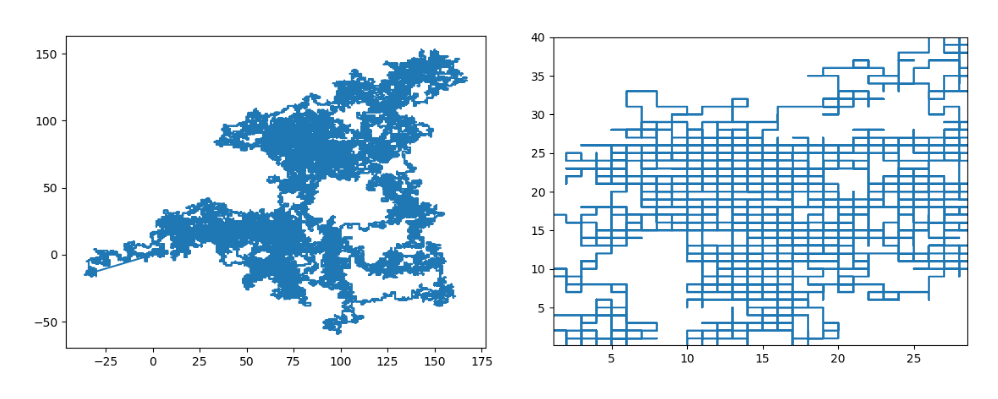
\includegraphics[scale=0.5]{figs/simplewalk}

The image at left shows the full walk with 55574 steps while the right zooms in to reveal the underlying lattice structure. The fractal dimension of this motion is rather uninteresting. For $d=1$, the Hausdorff dimension is known to be 3/2 while it is 2 for $d \ge 2$ \cite{saberi11}. 

\section{Attracted random walkks}
Saberi (2011) propose an attracted random walk where the walker is predisposed attracted, with some attraction coefficient $\alpha$, toward the $xy$-plane from a three-dimensional lattice. At a lattice point $(x,y,z)$ the walker has six choices for movement: up, down, left, right, forward, backwards. Let $p = \frac{1}{\alpha + 5}$ and $q = \frac{1}{4 \alpha + 2}$. When the walker is not on the $xy$-plane, i.e. $z\not = 0$, the walker has probability $\alpha q$ to move toward the plane and $p$ for all other directions. When the walker is on the $xy$-plane, i.e. $z=0$, the walker will move left, right, forwards, and backwards with probability of $\alpha q$ and up or down (thus moving off the plane) with probability of $q$. When, $\alpha = 1$ this is a pure three-dimensional random walk but when $\alpha \to \infty$ this becomes a two-dimensional random walk on the plane. The walker begins at the origin. 

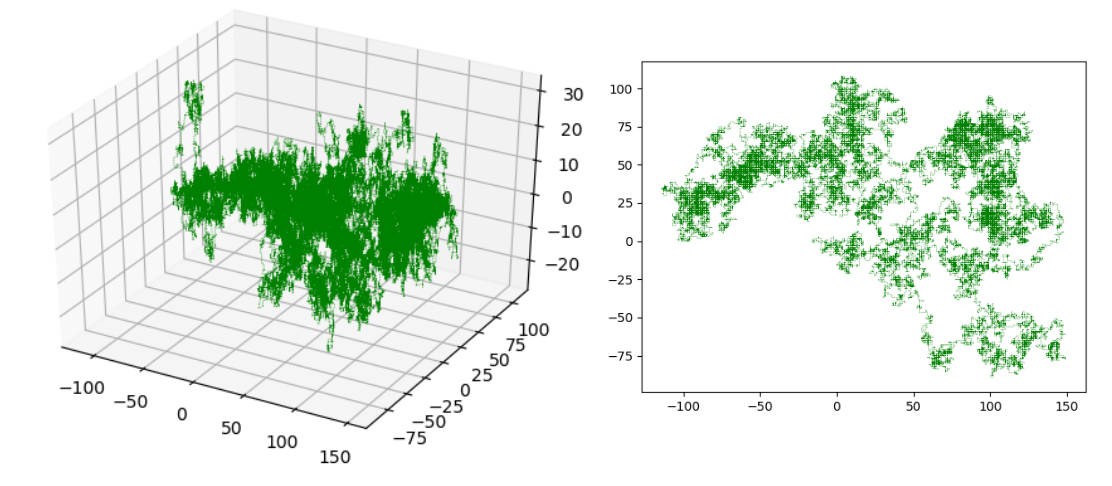
\includegraphics[scale=0.45]{figs/attracted3d}

Above is an example of this attracted random walk with $\alpha=1.3$ and $10^4$ steps. At left, you can see a side view in three dimensions and at right is the view directly from the top. This is lightly attracted. Below, you can see the result with $\alpha = 10$. 

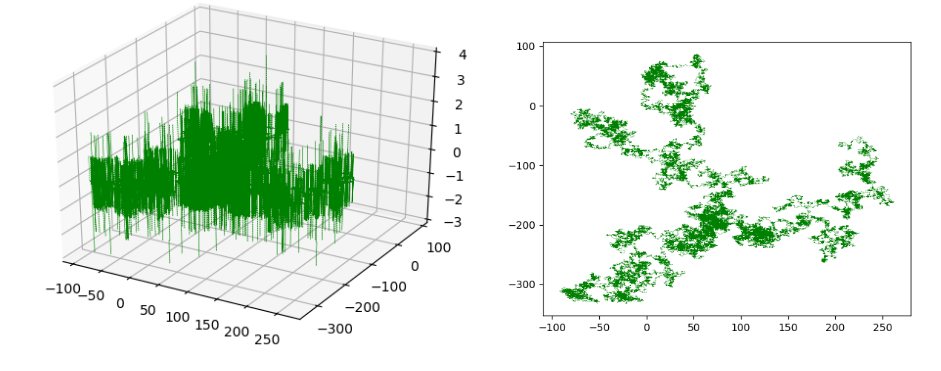
\includegraphics[scale=0.5]{figs/highlyattracted3d}

The walker can only get a few steps off the plane before it is pulled back onto it. Most of the interesting behavior occurs in this range of $1 < \alpha < 5$. However, by looking at very high $\alpha$ we can determine the limiting case. Saberi (2011) found this to be 1.83 \cite{saberi11}. However, I could not replicate this result. 

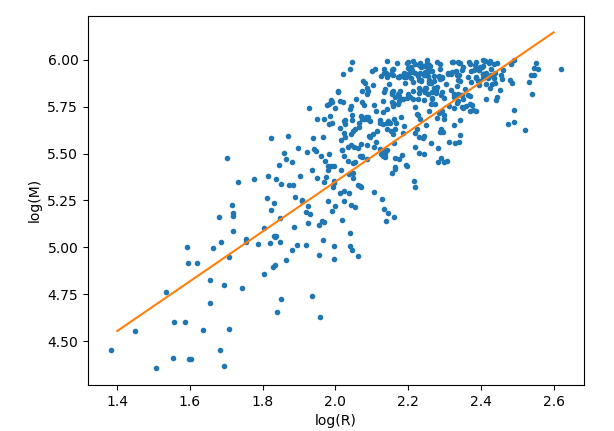
\includegraphics[scale=0.5]{figs/fit}

My fit line instead had slope of $1.3$. I did not have sufficient time to determine why this was different. 

\section{Code Contribution}
Since this project was computational, I will briefly outline my original code contributions. I have developed two independent software packages in Java: \jifs and \jwalker. These were kept separate as \jifs is being developed as a portable Java version of \href{https://www.matheasel.com/terafractal/mac/}{TeraFractal}, a beautiful fractal generation tool exclusively for Mac. \jifs provides iterated function systems in Java and measuring the Minkowski dimension while \jwalker handles the random walks portion. This report will be made available with the \jwalker code.

\subsection{jWalker}
This package includes the random walk code. It implements a simple arbitrary topological dimension point which is used by a generic random walk class. Then, I have implemented simple random walks as well as a plane attracted random walk. The random walk classes provide measurement tools for their dimensions. 

\subsection{\jifs}
This package has support for simple iterated function systems of affine transformations. It also supports visualizing them and has the capacity to add other kinds of iterated function systems. It provides support to measure the Minkowski dimension of a set of points. 

\section{Summary}
Ultimately, I was a bit disappointed with my result. I had planned (and still do) to explore more random walks. For example, I was planning on adding "traps" to the attracing plane where it was difficult to esacpe, or similarly points that pushed away dramatically. I was also planning on exploring it in higher dimensions and also constraining it so the walk could not go below the plane. I sketched out a version where instead of an attracting plane there was an attracting surface. However, I had insufficient time to implement. Another plan was to allow the walk to be attracted to an iterated function system instead of a plane. Thus, it would be offered "neighbors" that were from the IFS as well spatial neighbors. I thought it would be interesting to see the attraction. I had plans to allow for the attraction to depend on the distance from the plane as well, as simple modification (which shouldn't have resulted in much change if you were already on the plane except for an occasional wandering off). 

However, I had very little time with other finals and thesis work (I did apply fractal dimension in it though to find the fractal dimension of active regions on the Sun). I'm attaching an appendix with the code generated for this project (some of it did not get used because I ran out of time). I will return to this project after graduation and update this report with new results as they become available for your reading. 

\newpage

\bibliographystyle{acm}
\bibliography{references}

\newpage

\singlespace
\begin{appendices}
  \section{Code}
  I included copies of the code here for your easy of viewing. 
  
  \subsection{Point}
  \inputminted{java}{../src/Point.java}

  \subsection{RandomWalk}
  \inputminted{java}{../src/RandomWalk.java}

  \subsection{PlaneAttracted3D}
  \inputminted{java}{../src/PlaneAttracted3D.java}

  \subsection{Simple2D}
  \inputminted{java}{../src/Simple2D.java}
  
  \subsection{Simple3D}
  \inputminted{java}{../src/Simple3D.java}

  \subsection{plotFig1}
  \inputminted{python}{../src/plotFig1.py}
  
  \subsection{IFS}
  \inputminted{java}{/home/marcus/grive/codedungeon/jifs/src/IFS.java}
  
  \subsection{AffineTransform}
  \inputminted{java}{/home/marcus/grive/codedungeon/jifs/src/AffineTransform.java}
  
  \subsection{LinearRegression}
  \inputminted{java}{/home/marcus/grive/codedungeon/jifs/src/LinearRegression.java}
  
  \subsection{Matrix}
  \inputminted{java}{/home/marcus/grive/codedungeon/jifs/src/Matrix.java}
  
  \subsection{IFSEvaluator}
  \inputminted{java}{/home/marcus/grive/codedungeon/jifs/src/IFSEvaluator.java}
  
  \subsection{MinkowskiDimension}
  \inputminted{java}{/home/marcus/grive/codedungeon/jifs/src/MinkowskiDimension.java}
  
  \subsection{Transform}
  \inputminted{java}{/home/marcus/grive/codedungeon/jifs/src/Transform.java}
  
  \subsection{RandomIFSEvaluator}
  \inputminted{java}{/home/marcus/grive/codedungeon/jifs/src/RandomIFSEvaluator.java}
  
\end{appendices}


\end{document}
